\section{Alarm data transmission: remote monitoring module}
\label{scenario:rm-alarm}

\npar Figure \ref{fig:scenario-5-9} shows a sequence diagram for the ``Alarm
data transmission: remote monitoring module'' scenario. For every incoming
alarm trame, the trame is checked for a false positive by the anomaly detection
unit (only the case of a real alarm is shown), the valve is shut and the alarm
recipients are notified.

\begin{figure}[H]
	\begin{centering}
		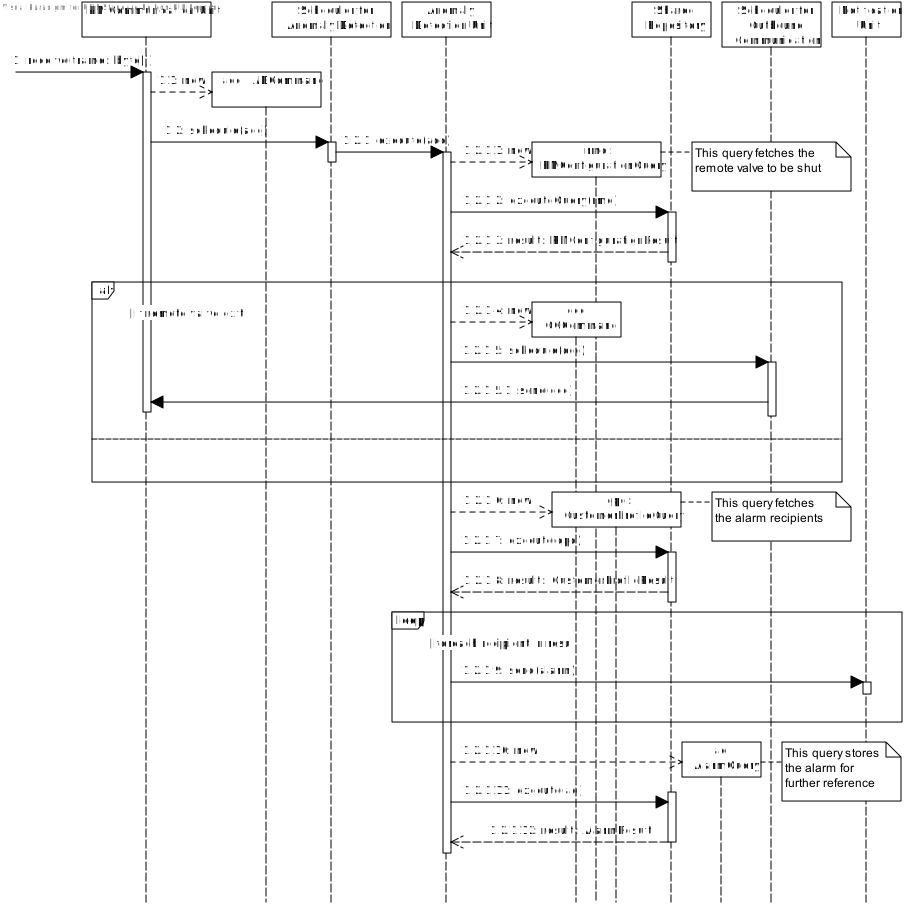
\includegraphics[width=\textwidth]{figs/scenario-5-9.pdf}
		\caption{Sequence diagram for the ``Alarm data transmission: remote monitoring
		module'' scenario}
		\label{fig:scenario-5-9}
	\end{centering}
\end{figure}